\documentclass[10pt, twocolumn]{article}

\usepackage{report}

\usepackage[utf8]{inputenc} % allow utf-8 input
\usepackage[T1]{fontenc}    % use 8-bit T1 fonts
\usepackage[colorlinks=true, linkcolor=blue, citecolor=blue, urlcolor=blue]{hyperref}       % hyperlinks
\usepackage{url}            % simple URL typesetting
\usepackage{booktabs}       % professional-quality tables
\usepackage{amsfonts}       % blackboard math symbols
\usepackage{nicefrac}       % compact symbols for 1/2, etc.
\usepackage{microtype}      % microtypography
\usepackage{lipsum}		    
\usepackage{graphicx}
\usepackage{footnote}
\usepackage{doi}
\usepackage{comment}
\usepackage{multirow}
\usepackage{gensymb}
\usepackage{float}
\usepackage{amsmath}
\usepackage{subfig}
\usepackage[skip=10pt plus1pt, indent=30pt]{parskip}

\begin{document}

\begin{titlepage}
    \centering
    %
\includegraphics[width=2.3cm]{crest.jpg}\par
    \vspace{1cm}
    {\scshape\Large Department of Physics and Astronomy \par}
    \vspace{1cm}
    {\scshape\Large The University of Southampton \par}
    \vspace{1cm}
    \vspace{1cm}
    {\huge\bfseries The Forced Simple Pendulum \par}
    \vspace{1cm}
    {\Large Ong Chin Phin (Linus) \par}
    \vspace{1cm}
    {\Large Student ID: 33184747 \par}
    \vfill
    {\large November 2023 \par}
\end{titlepage}

%\maketitle
\newpage
\onecolumn
\tableofcontents
\thispagestyle{empty}
\clearpage

\newpage
\thispagestyle{empty}
\begin{abstract}
%write wha tht experiment is about and what are the results 10-15 lines

%results go here
\end{abstract}

% keywords can be removed
%\keywords{First keyword \and Second keyword \and More}
\twocolumn
\newpage
\setcounter{page}{1}
\section{Introduction}
The forced simple pendulum looks, deceivingly simple. A bob on a string where the other end is attached to a fixed point is allowed to oscillate with an initial angular velocity experiences a damping force that acts against the pendulum - if the damping force (determined partly by a damping coefficient) is large enough, it will affect the motion of the oscillating pendulum. \\
\\
The equation of motion for a pendulum of a mass $m$ and length of $L$ is:
\begin{equation}
    mL^2 \frac{d^2\theta}{dt^2} + k \frac{d\theta}{dt} + mgL\sin({\theta}) = FL\cos({\Omega}t)
    \label{oscillation}
\end{equation}
Where:
\begin{itemize}
    \item $m$ is the mass of the pendulum bob
    \item $L$ is the length of the pendulum
    \item $\theta$ is the angular displacement of the pendulum from vertical
    \item $\dot{\theta}$ is the angular velocity (rate of change of $\theta$)
    \item $\ddot{\theta}$ is the angular acceleration
    \item $k$ is the damping coefficient (dependent on the specific damping mechanism)
    \item $g$ is acceleration due to gravity
    \item $F$ is the magnitude of the external force
    \item $\Omega$ is the frequency of the external force $F$
    \item $t$ is the time
    \item $k\dot{\theta}$ is the damping force
\end{itemize}
\\
Since time is measured relative to the period of free oscillations of small amplitude, I can write:
\begin{equation}
    t = \tau\sqrt{\frac{L}{g}}
    \label{modified time}
\end{equation}
And:
\begin{equation}
    \Omega = (1 - \eta)\sqrt{\frac{g}{L}}
    \label{modified omega}
\end{equation}
To investigate the situation where the behavior of the pendulum when the forcing frequency, $\Omega$ is slightly less than the natural frequency, $\frac{g}{L}$.
\\
\\
In the following sections, I introduce the method on how to change the 2nd order differential equation Eqn. (\ref{oscillation}) into a matrix equation in the form of $\vec{\bold{Y'}} = A\vec{\bold{Y}} - \vec{\bold{b}}$, such that they can be solved numerically using the Runge-Kutta method.
\\
\\
I will then investigate various scenarios, which will be introduced at the end of the Methodology section. Results are then compared to known data.
\\
\\
The Rayleigh-Lorentz pendulum \cite{Rayleigh1902}, named after Lord Rayleigh and Hendrik Lorentz, is a simple pendulum where the forcing frequency is changing due to the change of the pendulum length\footnote{It has been shown that from \cite{Rayleigh1902}:
\begin{equation}
    \frac{E(t)}{f(t)} = \frac{E(0)}{f(0)}
\end{equation}
Stating that the ratio of average energy to frequency is constant. This is an example of an adiabatic invariant - meaning that it is a conservation law that stays constant only when changes to the parameters are done slowly. }. With the forced simple pendulum, I investigate the effects on the forced simple pendulum with a changing length. The case of a uniform and exponential change in the pendulum length have been investigated in the case of a simple pendulum in \cite{Brearley1966, Werner1969, Ross1979} (for a uniform change) and \cite{SanchezZoido2013} (for both uniform and exponential), where the linear variation was determined by the equation $l(t) = l_0 (1 + \epsilon{t})$, and the exponentially varying case is given by the equation $l(t) = l_0\exp{\epsilon t}$. Where $\epsilon$ in both equations is a small parameter of unit $s^{-1}$. There are many other variations that I can investigate, for example a sinusoidal (or simply a periodic) variation, a non-linear (quadratic or higher order) variation, or even a random variation (Brownian motion or random walks). A random walk is an interesting option for a number of reasons:
\begin{itemize}
    \item Real world systems are experience random fluctuations. For example, a skyscraper or bridge will not experience a constant force.
    \item Stability of the pendulum system could be assessed. What is the optimum pendulum (one that is resilient to random changes in forces)?
    \item Resonant frequencies can be identified easily
    \item Long term behaviour prediction
\end{itemize}

\section{Methodology}
To convert equation (\ref{oscillation}) into dimensionless form, we recall that: $t = \tau\sqrt{\frac{L}{g}}$  and by the chain rule, $\frac{d\tau}{dt} = \frac{d\theta}{dt}\frac{dt}{d\tau}$ give the following equations:
\begin{equation}
    \begin{split}
        \frac{d\theta}{dt} = \sqrt{\frac{g}{L}}\frac{d\theta}{d\tau} \\
        \frac{d^2\theta}{dt^2} = \frac{g}{L}\frac{d^2\theta}{d\tau^2}
    \end{split}
    \label{chain rules}
\end{equation}
Which can be substituted into equation (\ref{oscillation}) after dividing by $mgL$ and substituting equation (\ref{modified time}) and (\ref{modified omega}).
\begin{equation}
        \centering
        \begin{split}
            & (\frac{L}{g})(\frac{g}{L})\frac{d^2\theta}{d\tau^2} + \frac{k}{mgL}\sqrt{\frac{g}{L}}\frac{d\theta}{d\tau} + \sin(\theta)\\
            & = \frac{F}{mg}\cos((1 - \eta)\sqrt{\frac{g}{L}}\sqrt{\frac{L}{g}}\tau)
        \end{split}    
\end{equation}
The dimensionless form of equation (\ref{oscillation}) is then:
\begin{equation}
    \frac{d^2\theta}{d\tau^2} = -\alpha\frac{d\theta}{d\tau} - \sin(\theta) + \beta\cos((1 - \eta)\tau)
    \label{dimensionless}
\end{equation}
With parameters\footnote{
    Note that:
    \\
        \begin{equation}
            \frac{k}{mgL}\sqrt{\frac{g}{L}} = \frac{k}{mL\sqrt{g}\cdot\sqrt{g}}\sqrt{\frac{g}{L}} = \frac{k}{mL\sqrt{gL}}
        \end{equation}
}: 
\begin{equation}
    \centering
    \begin{split}
        \alpha &= \frac{k}{mL\sqrt{gL}}\\
        \beta &= \frac{F}{mg}
    \end{split}
    \label{parameters}
\end{equation}
The RK4(5) (Runge–Kutta–Fehlberg) method will be used to solve the equation numerically. I will be using \verb|scipy.integrate.RK45| that uses the Dormand-Prince pair of formulas \cite{DormandPrince1980}. To solve a 2nd order differential equation with any Runge-Kutta method, the ODE in question will have to be expressed as a 1st order ODE. 
From equation (\ref{dimensionless}) and taking the substitution:
\begin{equation}
    \omega = \frac{d\theta}{d\tau}
\end{equation}
The ODE will be a system of equations of the form $\vec{\bold{Y'}} = A\vec{\bold{Y}} - \vec{\bold{b}}$.
\begin{gather}
    \begin{bmatrix}
        \theta' \\ 
        \omega'
    \end{bmatrix}
    =
    \begin{bmatrix}
        0 & 1 \\
        $-\sin(\theta)$ & $-\alpha$
    \end{bmatrix}
    \begin{bmatrix}
        \theta \\ 
        \omega
    \end{bmatrix}
    -
    \begin{bmatrix}
        0 \\
        $\beta\cos((1 - \eta)\tau)$        
    \end{bmatrix}
\end{gather}

\section{Setup}\label{setup}
The code used for the entirety of the project can be found on my \hyperlink{https://github.com/linsuong/PHYS-6017-Labs/blob/main/Projects/ForcedSimplePendulum}{GitHub page}. 
\\
\\
First, I think it is useful to have a rough understanding on the effects of each parameter on the numerical solution of the pendulum. By giving the constants values and altering each one, I can (without complete certainty, of course) predict the pendulum behaviour for later experiments.
The system is set up as follows:
\begin{itemize}
    \item The pendulum has a mass $m$ of 1kg
    \item The length of the string, $L$ is 2 meters
    \item The damping coefficient $k$ has a value of 10
    \item The factor $\eta$ has a value of 0.1
    \item $g$ is 9.81$ms^{-1}$
    \item Time interval is 0 to 50 seconds \footnote{As the RK4(5) algorithm goes for longer, the errors stack up. It is not wise to use a long time interval at once without taking any precautions. Therefore a relatively short time period is investigated.}
\end{itemize}
By modifying each parameter, I plot the time-domain ($\theta$ against $t$) and the phase portrait\footnote{See Section \ref{phase plots appendix} for an explanation on phase portraits, as this is not covered in any core module.}  Each notable simulation will contain a time-domain plot and a phase portrait plot ($\frac{d\theta}{dt}$ against $\theta$). 

\onecolumn
\begin{figure}[H]
    \centering
    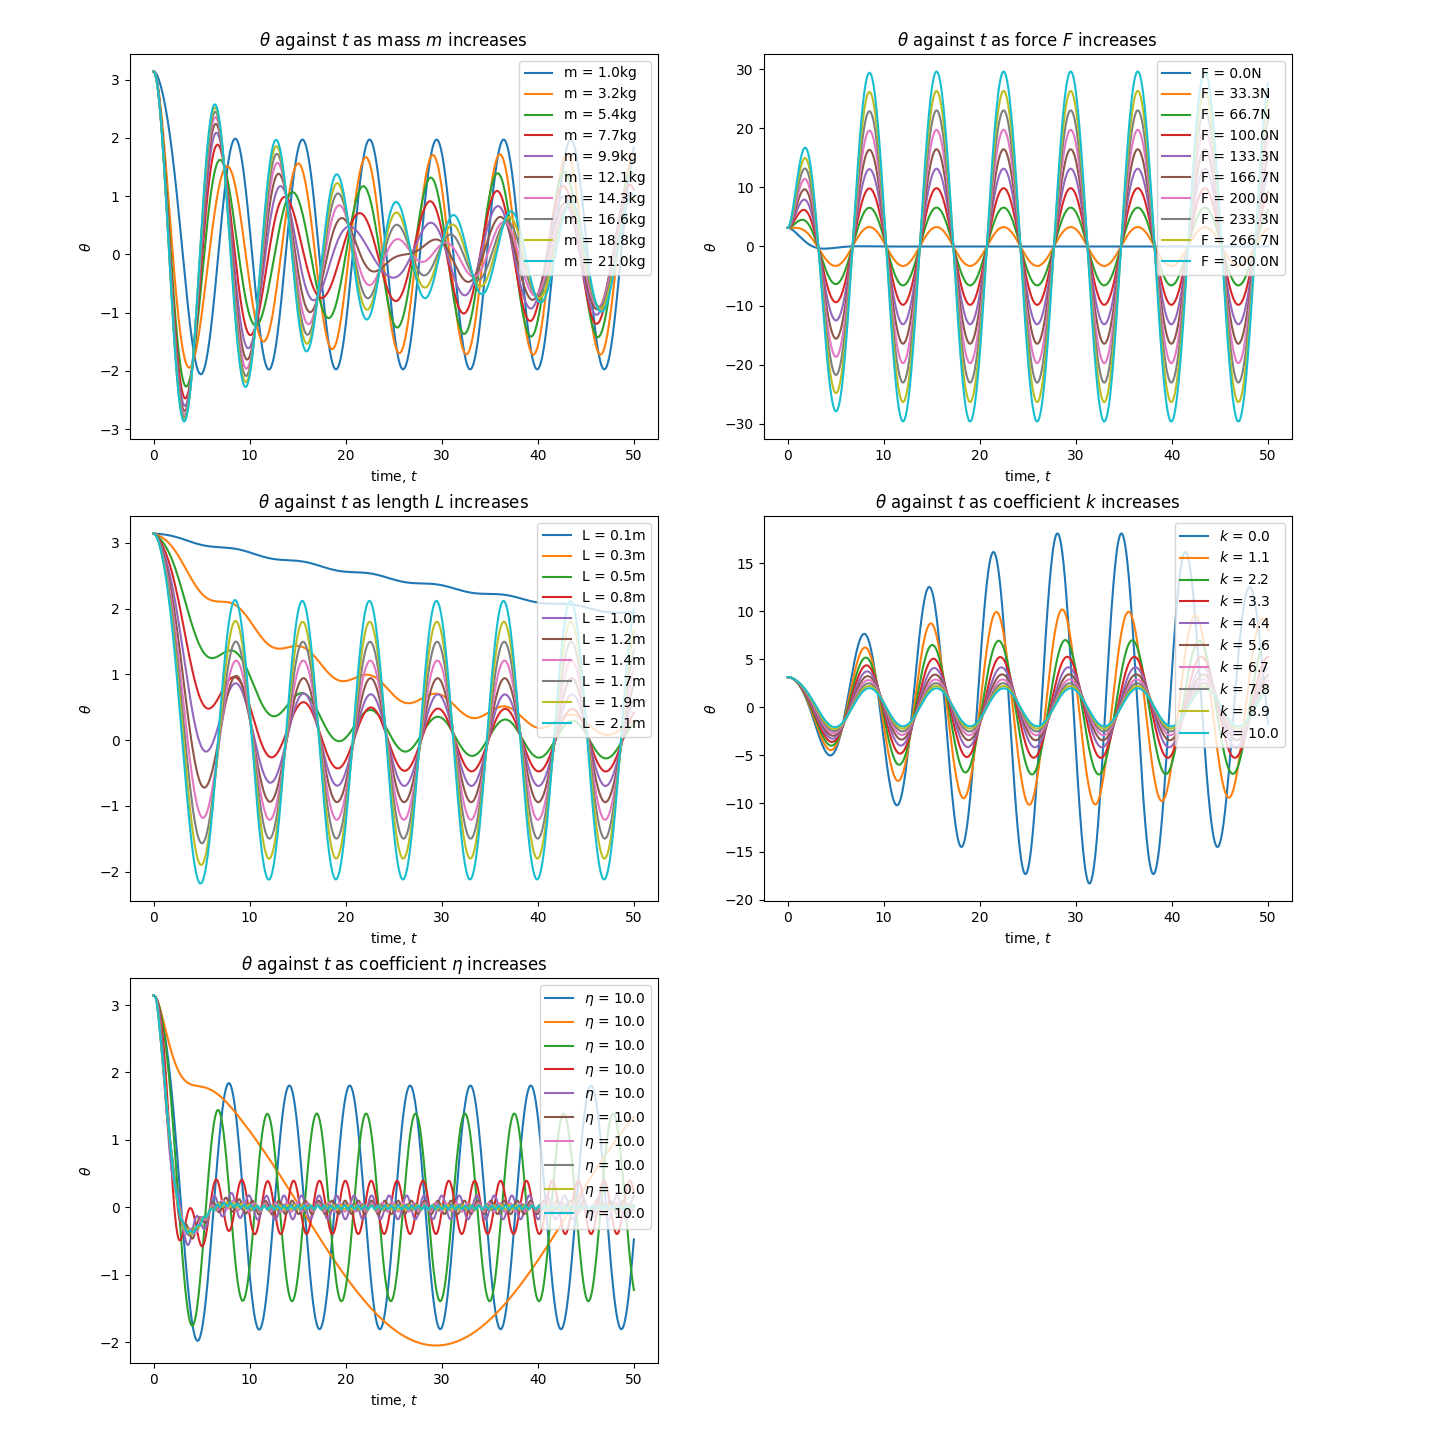
\includegraphics[width = 1.1\columnwidth]{Projects/ForcedSimplePendulum/Plots/test_plots.png}
    \caption{Time-domain plots for the case of the simple forced pendulum, where each variable is iterated one by one.}
    \label{time domain test}
\end{figure}

\begin{figure}[H]
    \centering
    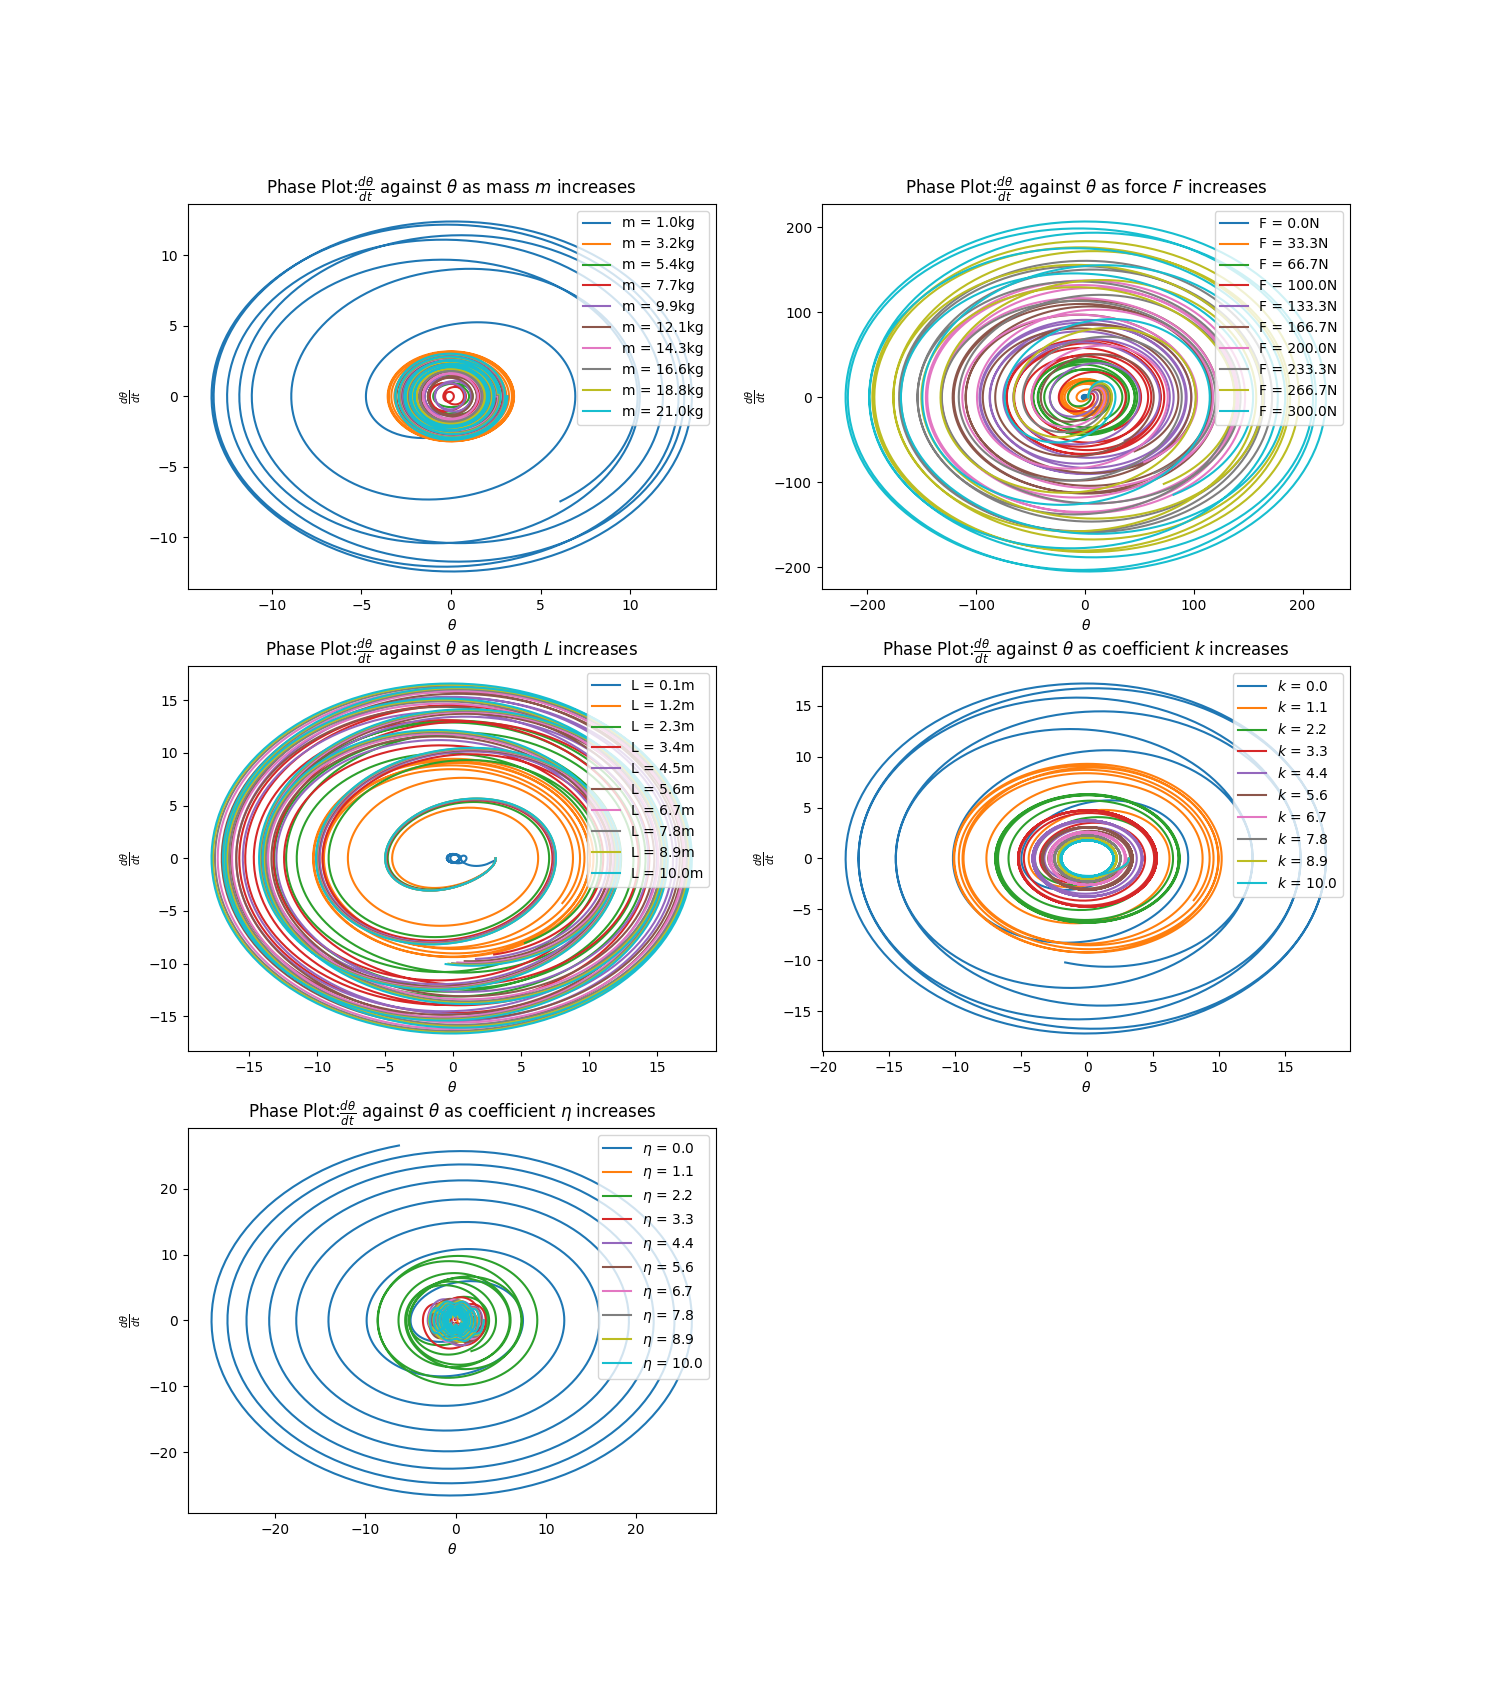
\includegraphics{Projects/ForcedSimplePendulum/Plots/test_plots_phase.png}
    \caption{Phase portraits for the case of the simple forced pendulum, where each variable is iterated one by one.}
    \label{phase portrait}
\end{figure}

\twocolumn
\section{Areas of Investigation}
The areas of investigation are:
\begin{itemize}
    \item When the force, $F$ is almost equal to the weight of the pendulum bob, $mg$. Damping is reduced till a change is observed.
    \item When the force, $F$ is much greater than the weight of the pendulum bob (extreme forcing). Periodic motion is observed in this scenario. I investigate when the periodic motion is gone as I decrease $F$.
    \item General behavior for 0 damping, where I investigate scenarios where 'beats' are seen between the natural period and the forcing period.
\end{itemize}
 
\subsection{Simple Forced Pendulum}
First, I investigate the case on where $F \sim{mg}$. With the same values of the other constants in Section \ref{setup}, with the exception of $F = 9.81N$ and iterating over values of $k$ from 
\begin{figure}[H]
    \centering
    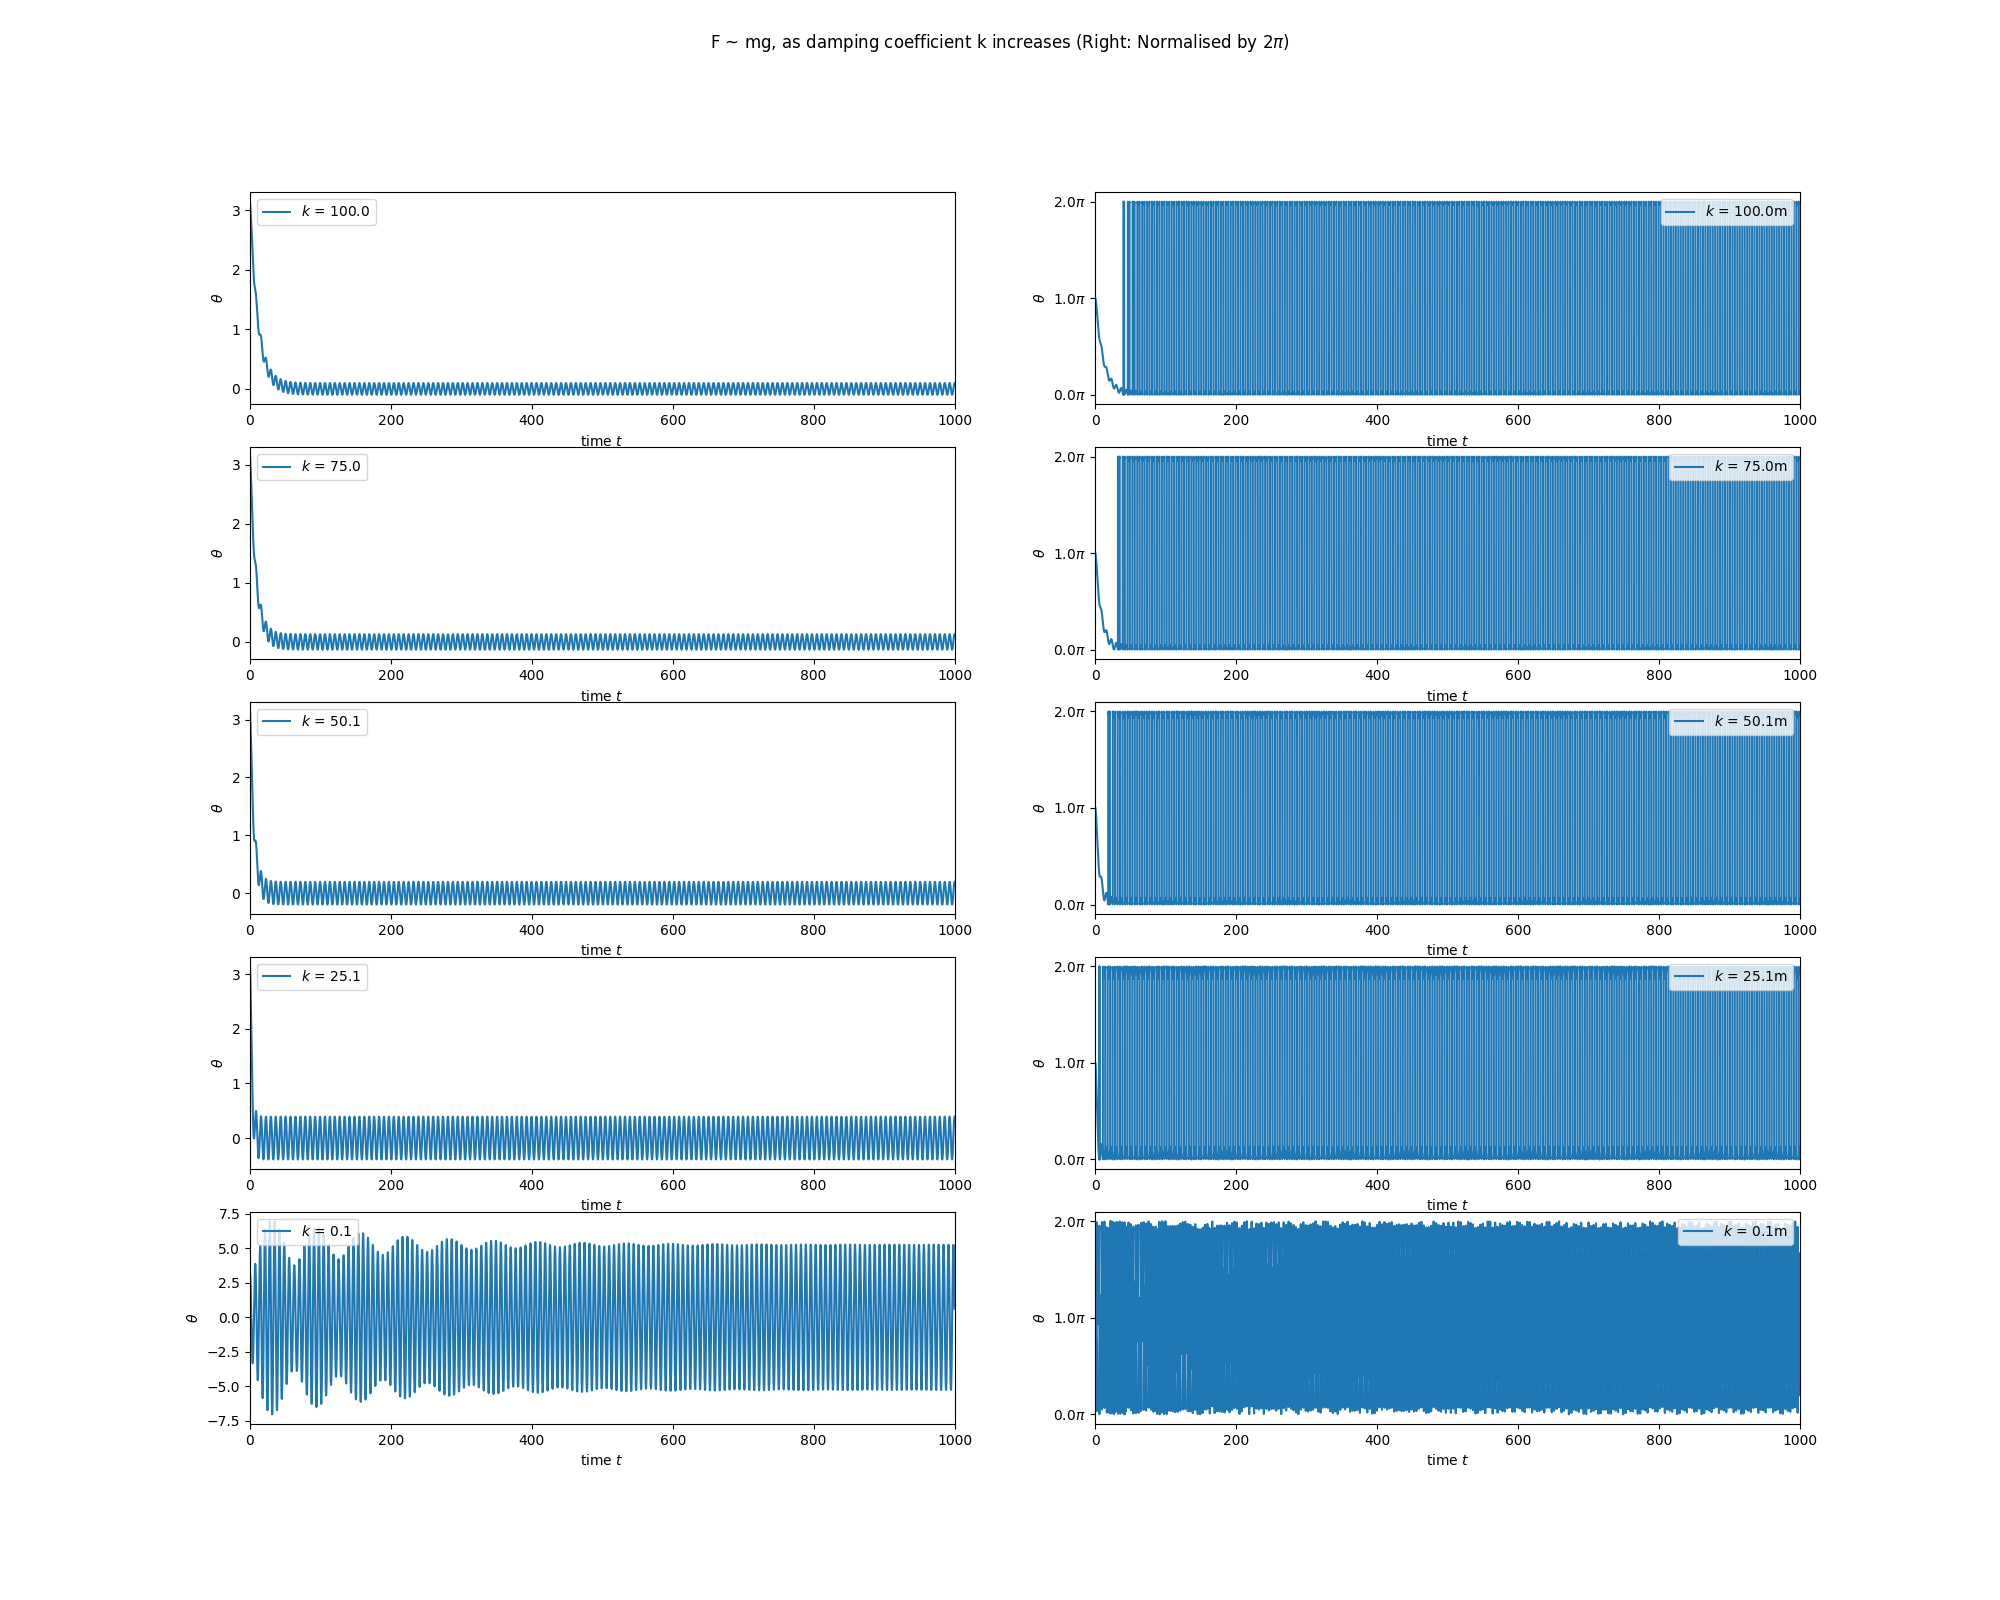
\includegraphics[width =\columnwidth]{Projects/ForcedSimplePendulum/Plots/F~mg as damping coefficient k increases.png}
    \caption{Time-domain plot for the forced simple pendulum as k is increased. (Left column: raw data; Right column: data normalised by $2\pi$}
    \label{fig:enter-label}
\end{figure}

\subsection{Rayleigh-Lorentz Pendulum}


\section{Results}

\section{Analysis}
\section{Conclusion}

\subsection{Future Work}
Future work could involve extending the Rayleigh-Lorentz pendulum to the case of a double pendulum, or investigating a sinusoidal change in length (for the case of a single and double pendulum). 
\newpage
\section{Addendum} %complete
This section outlines 3 concepts studied in PHYS6017, namely random walks, Monte Carlo simulations, and random walks. A brief description of each concept is stated before some examples in and out of academia are given.
%stuff here
%Show you understand the basics of the technique
% Give 6 examples (including proper references), where the technique has been used in:
% 3 in Academia…
% 3 Outside academia (industry, medicine, finance, etc)
\subsection{Random Walks} %complete
Random walks are a way to generate data. A simple example would be the case of a particle on a 2-D plane, where the particle is allowed to move in one of the four directions possible, and the choice of direction is random, usually according to some probability distribution.

\subsubsection{In Academia} %complete
In \cite{Kruzins1982}, by knowing the sound intensity at a few detection points, sound fields (more specifically, the steady state high frequency SPL) in non-diffuse spaces can be predicted via random walks, built upon \cite{Gerlach1975}. Random walks have been used in biophysics for an algorithm reconstructing supercoiled DNA \cite{Baba2020} (supercoiled meaninng the amount of "twist" in a DNA strand, thereby giving the magnitude of strain on it) \cite{Bauer1980}. The DNA is found to take a random walk, which can be tied to the travelling salesman problem. Furthermore, mapping random walks onto complex network structures (where the moving probability is taken as information flow), and \cite{Noh2004} discovered that information had a directional flow (when random walks were mapped), as opposed to a bidirectional flow (along the backbone of a network). 

\subsubsection{Outside of Academia} %complete
Random walks were used in cybersecurity, where cyber threats were detected via a "self-avoiding" (random) walk \cite{Nia2016}. The patterns were extracted and compared to a threat database. Random walks were also used to predict pedestrian and vehicular movement in London \cite{Hanna2021}, and proved to be very effective, compared to a segment-based centrality measures \cite{Jayasinghe2015}. A random walk was also used in a simple risk business \cite{Seal1966}, seeing the probability of ruin as the number of contracts go up.

\subsection{Monte Carlo Simulations} %complete
Prevalent in the world of finance, physics, engineering, statistics and many more, the famous casino in Monte Carlo was inspiration to the Monte Carlo simulation. It is a way to solve complex problems typically involving many variables, which may be challenging to solve analytically. They rely on randomness to generate large numbers of outcomes via simulations, where probabilities or expectation values can be calculated.

\subsubsection{In Academia} %complete
The Monte Carlo (MC) method was used to do a simulation of the Ising model in in 2-D \cite{Shekaari2021}\cite{Jindal2007}, a very important model in statistical mechanics. It is also used in robotics, where it is used to improve localisation of a moving robot in a dynamic enviroment \cite{Zhao2008} by using a vision-based MC localization. MC method is also used in machine learning for gradient estimation - the pathwise, score function and measure-valued gradient estimators were used \cite{Mohamed2020}.

\subsubsection{Outside of Academia} %complete
Many applications were developed for proton therapy using the Monte Carlo method, such as VMCpro \cite{FippelSoukup2004} (patient dose calculation), MCNPX \cite{Waters2002}, FLUKA \cite{Ferrari2005} and Geant4 \cite{Geant4} \cite{Geant4_2} (all-particle code that can work with motion and magnetic fields). TOPAS (TOol for PArticle Simulation) \cite{Perl2012}\cite{Faddegon2020} was then developed using the Geant4 toolkit to make it more accessible to medical physicts, radiobiologists and clinicians. Other than proton therapy, MC method is used in risk analysis of the energy efficiency investments in buildings \cite{Togashi2019}, by calculating probability distribution of energy reduction. MC method is also used in quality control \cite{Moran2023}. The important characteristics of a product can be identified, allowing the manufacturer to prioritise certain aspects of their product to ensure customer satisfaction.

\subsection{Random Numbers} %complete
Random numbers are numbers generated randomly where the current number generated has no relationship to the previous number generated, and neither will the current number have an effect on the next. They are used extensively in fields such as cryptography and statistics.

\subsubsection{In Academia}
An efficient stock market resembles a random number generator \cite{Doyle2013}. Therefore, random numbers were used to test the Efficient Market Hypothesis (EMH) \cite{Yen2008} by using the Overlapping Serial Test \cite{Good1953}, a form of test for randomness. Randomised numerical linear algebra \cite{Martinsson2020} could be applied into statistics \cite{Gentle2012}. Random numbers have been used in investigating access games by having a random number of players \cite{Tembine2008}.

\subsubsection{Outside of Academia} %complete
True random number generators (TRNG), as outlined in \cite{Sunar2009} are used in cryptography (where the TRNG has to meet certain criteria \cite{Latham2001}). TRNG was also used in audio encryption \cite{Etem2020}. Following the (not so recent) cryptocurrency boom, blockchain-based random number generators \cite{Hsieh2022} are explored and their uses in blockchain games \cite{Du2019}. Random numbers are also used in clinical trials \cite{Beller2002}, which assign participants to either of the available groups (i.e. a placebo and non-placebo group for a vaccine test).

\newpage
\section{Bibliography}
\bibliographystyle{apalike}
\bibliography{references}

\onecolumn
\newpage
\section{Appendix A}
\subsection{Phase Plots (or Phase portrait)} \label{phase plots appendix}
Phase plots (meaning plot of $\frac{d^2\theta}{dt^2}$ against $\frac{d\theta}{dt}$ in this case), are different from the usual time-domain plots ($\theta$ against t). The classic time-domain plot is a good way to visualise the change of the pendulum's position over time. The time-domain plots give the oscillation period (thereby the frequency), amplitude, and it is easy to see if any damping/external forces have been applied onto the system (the pendulum). A phase portrait, on the other hand give visualisation of the system's evolution in phase space. The intersection of trajectories at a point (or the approach of trajectories to a point) can indicate equilibrium points, stability (via attractors or repellers), limit cycles (repeated behaviour) or chaotic behaviour.
\begin{figure}[H]
    \centering
    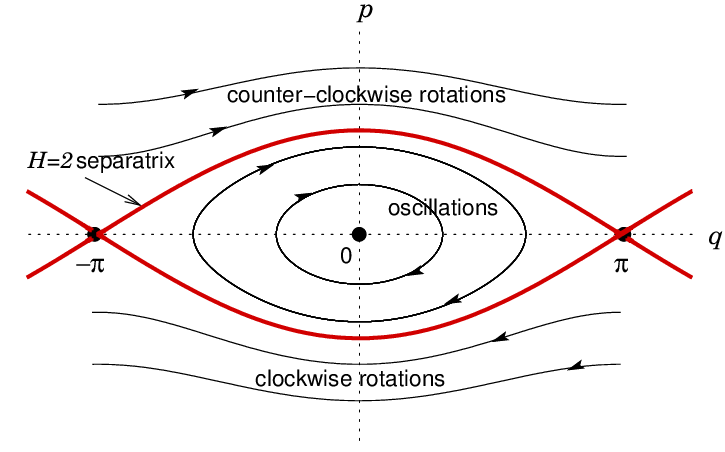
\includegraphics[width = 0.7\columnwidth]{Projects/ForcedSimplePendulum/WrittenReport/figs/The-phase-space-of-the-simple-pendulum.png}
    \caption{Phase plot for a simple pendulum. Taken from \cite{Ball2007}.}
    \label{fig:enter-label}
\end{figure}

\begin{figure}[H]
    \centering  
    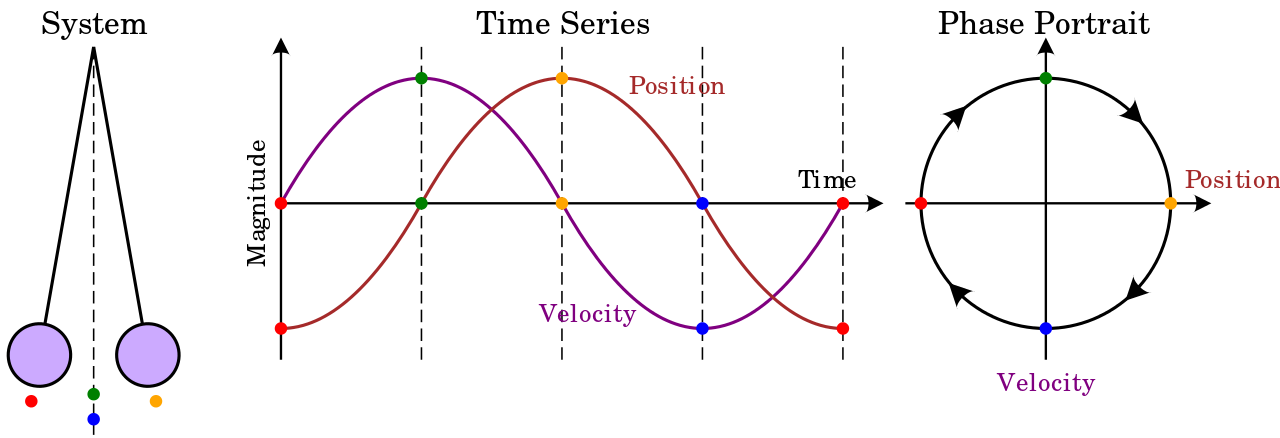
\includegraphics[width = \columnwidth]{Projects/ForcedSimplePendulum/WrittenReport/figs/Pendulum_phase_portrait_illustration.svg.png}
    \caption{How a phase portrait is compared to a time-domain plot for a simple pendulum. The blue dot for the illustration of the system corresponds to the blue dots on the time series graph and the phase portrait (and so do the other coloured dots). Taken from \hyperlink{https://commons.wikimedia.org/wiki/File:Pendulum_phase_portrait_illustration.svg}{WikiMedia}.}
    \label{fig:enter-label}
\end{figure}
 It is useful to consider both plots for this project. I will introduce some simple examples of the comparison of time-domain and phase-domain plots.
 \begin{figure}
     \centering
     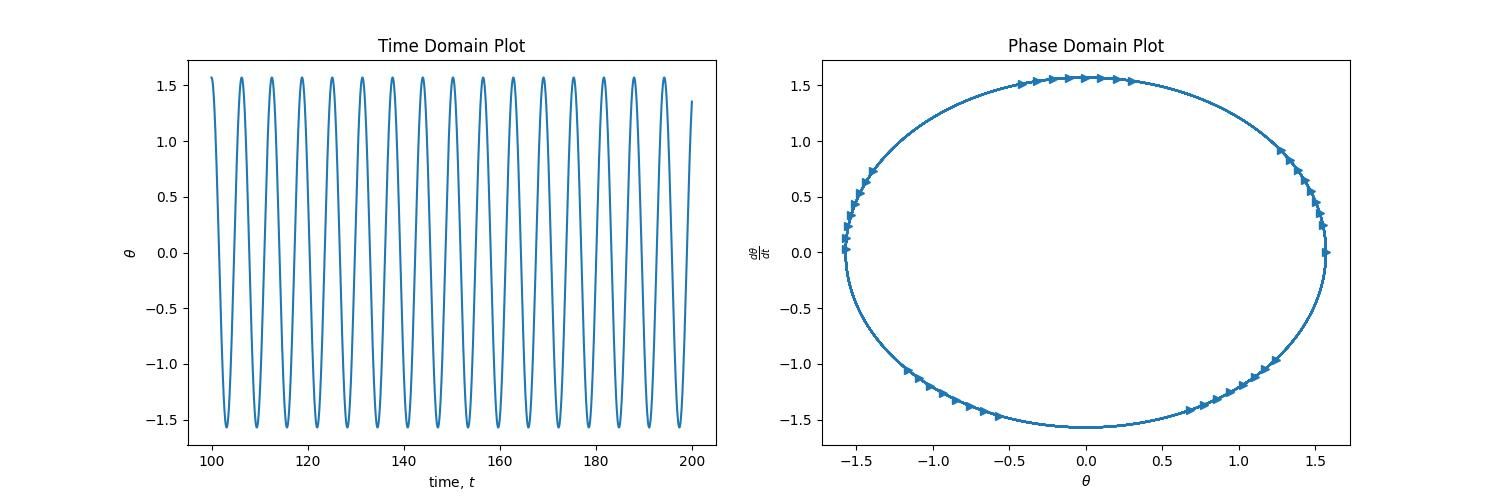
\includegraphics{Projects/ForcedSimplePendulum/Plots/demo_simple_harmonic_motion.jpg}
     \caption{Time and Phase domain plots for simple harmonic motion.}
     \label{fig:enter-label}
 \end{figure}

 \begin{figure}
     \centering
     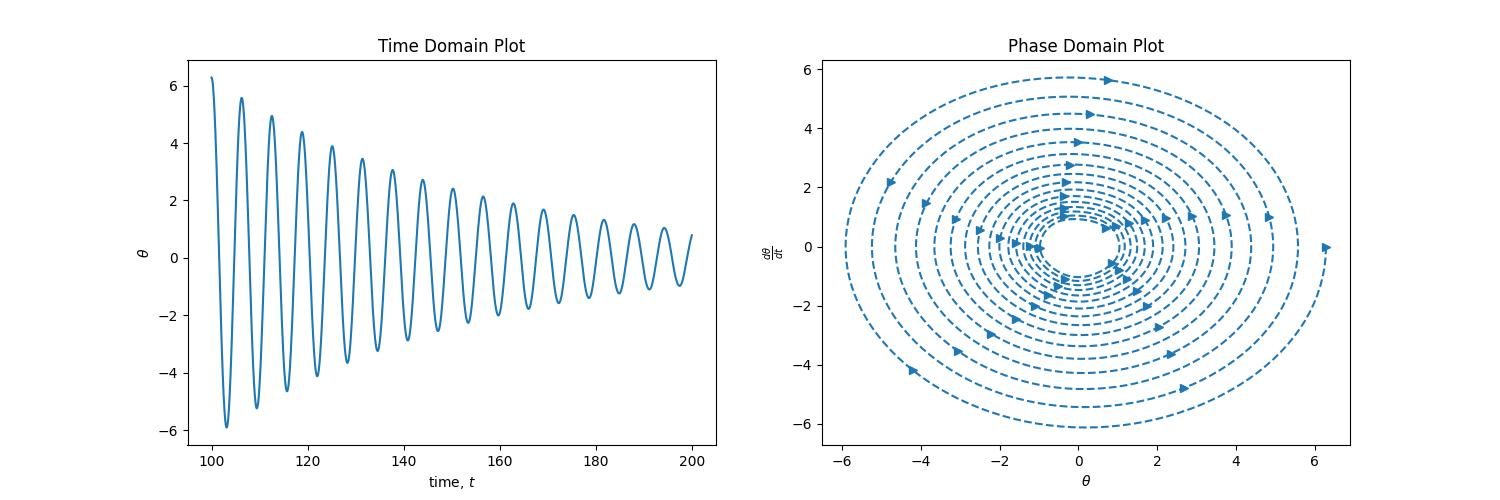
\includegraphics{Projects/ForcedSimplePendulum/Plots/demo_limit_cycles.jpg}
     \caption{Due to the presence of damping (seen in the time-domain plot), these plots showcase the concept of limit cycles (in the phase-domain plot), where trajectories spiral into each other.}
     \label{fig:enter-label}
 \end{figure}

\begin{figure}
    \centering
    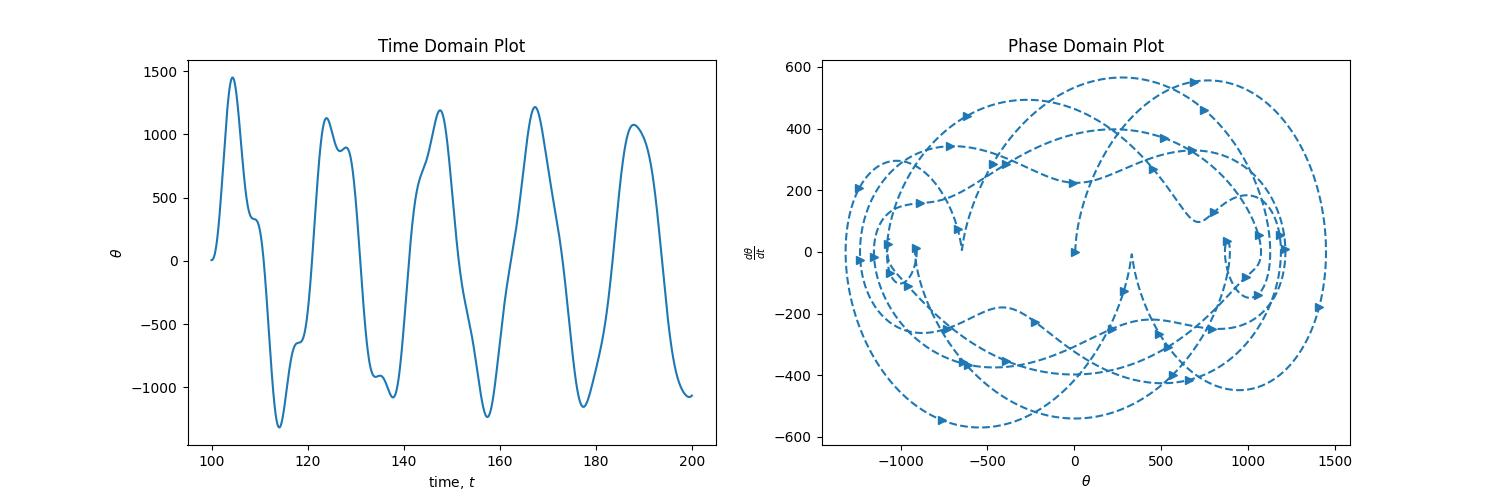
\includegraphics{Projects/ForcedSimplePendulum/Plots/demo_chaos.jpg}
    \caption{An example of chaotic behaviour. It definitely would not have been obvious just by looking at the time-domain plot alone.}
    \label{fig:enter-label}
\end{figure}

\section{Appendix B}
The plots

\end{document}